\documentclass[12pt]{article}
\usepackage{lipsum} 
\usepackage{graphicx}
\usepackage{geometry}

\graphicspath{ {./images/} }
\geometry{
    left=2.5cm,
    right=2.5cm,
    top=3cm,
    bottom=3cm
}
\usepackage[ngerman]{babel}

\title{Roboterschwarm}
\begin{document}

     \section*{Controller für Autonome Roboterschwärme}
    Ausarbeitung zum Thema:\\Distributed deformable configuration control for multi-robot systems with 
    low-cost platform
    \\von Seoung Kyou Lee\\\\
    Fakultät für Mathematik und Informatik, Institut für Informatik\\
    Forschungsseminar Parallelverarbeitung, Wintersemester 2022/23\\\\
    Autor: Ferris Kleier\\
    Datum: 14. Februar 2023

    \section{Einleitung}

Die Arbeit beschäftigt sich mit dem Erkennen und Ausweichen von Hindernissen eines autonomen 
Roboterschwarms. Diese Roboter könne ihre Umgebung nicht selber wahrnehmen, sondern tasten Hindernisse als
Netz ab. Ziel dieser Arbeit ist es, einen Controller in Form eines Automaten zu entwicklen, durch welchen
die Roboter Umgehungsstrategien anwenden und sich ohne Verbindungsabbrüche im Raum bewegen können. Der
Schwarm agiert dabei dezentral, das heißt es gibt weder eine zentrale Steuereinheit, noch GPS oder 
Kartensysteme mit denen sich der Schwarm orientiert. Dieses Vorgehen kann kostengünstig und effizient
umgesetzt werden, da auch einzelne Roboter ausfallen können, ohne, dass der gesamte Schwarm ausfällt. Die
Roboter kommunizieren untereinander in einer Baumstruktur, Graphenalgorithmen sind für diese Arbeit also
ein essentieller Bestandteil. Nachdem die Roboter und ihr Aufbau als Schwarm vorgestellt werden, wird das
Herzstück dieses Controllers und der Phasenübergangsautomat behandelt. Am Ende werden Simulationsergebnisse
ausgewertet, um die Funktion des Controllers zu garantieren.

    \section{Der Roboter}

Diese Arbeit behandelt einen Roboterschwarm im zweidimensionalen Raum. Dabei hat sich der Autor für den 
R-One entschieden. Dieser besitzt 8 Infrarot-Sensoren zur Ermittlung von Nachbarn, zwei Räder um sich
auf dem Boden fortzubewegen, einen Prozessor, Speicher und einen Akku. Da die Infrarot-Sensoren ab einem
Meter stark an Genauigkeit abnehmen, werden die Roboter einen Abstand von weniger als einen Meter einhalten.
Die Sensoren eines Roboters $R_i$ teilen nun den umliegenden Raum in 16 Teile auf, um die Nachbarn anhand 
ihrer Lage und Ausrichtung zu $R_i$ zu speichern. In der Abbildung sieht man, wie die Sensoren den Raum
aufteilen. Nachbarn eines Roboters $R_i$ werden nun nach folgender Formel gespeichert:\\

$q_j^i=(x_j^i,y_j^i,\theta_j^i)=(d_{ij}\cos(b_j^i),d_{ij}\sin(b_j^i),b_j^i+\pi-o_j^i)$\\\\
Diese Formel speichert die Koordinaten und Ausrichtung eines Nachbarn, ausgehend von $R_i$ als Ursprung
eines Koordinatensystems. $x$ und $y$ bilden dabei die Koordinaten im Raum und $\theta$ die Ausrichtung.
Man kann die Position eines Nachbarn auch durch $d$, $b$ und $o$ speichern, wobei diese Formel einen Kreis
um $R_i$ mit Radius $d$ zieht, der Nachbar dann an der Stelle $b$ auf dem Kreis liegt und $o$ die
Ausrichtung zu $R_i$ angibt. Im zweiten Verfahren werden alle Werte in Grad gemessen. Die Ausrichtung eines
Nachbarn zu $R_i$ ermittelt sich übrigens daraus, welche Sensoren ausgehend vom 'Kopf' des Roboters
angesprochen werden. Die Roboter erkennen so den Winkel der Ausrichtung durch Abgleichen der ID ihrer
Sensoren.\\

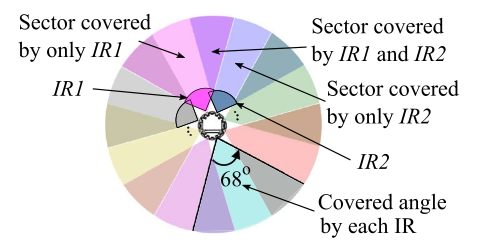
\includegraphics[width=2.5in]{images/Screenshot 2023-02-16 at 11.53.03 AM.png}\\\\
Die Roboter tauschen nun ständig im Millisekundentakt ihre Nachbarn aus und speichern diese als Array.
Als nächstes betrachten wir, wie mehrere solcher Roboter einen Schwarm bilden.

    \section{Schwarmaufbau}

    \section{Der Controller}

Folgende Gleichung bildet das Herzstück der Arbeit, den eigentlichen Controller:\\

$u_i^\alpha=\sum\limits_{R_j\in N_i^1}\phi_\alpha(||q_j^i||_\sigma)n_{ij}^i+
\sum\limits_{R_j\in N_i^1}p_j^i$\\\\
Diese Gleichung, die Alpha-Control, ist nur ein Teil einer Summe mehrerer Controls. Da die anderen beiden
(Beta- und Gamma-Control) jedoch auf zentralisierte Methoden beruhen, werden diese für die Arbeit nicht
betrachtet. Die Alpha-Control gibt einfach ausgedrückt die Distanz und Ausrichtung zwischen Robotern an,
die eingehalten werden muss, um aus dem Schwarm ein Dreieck-Gitter mit gewünschter Größe zu machen, 
ähnlich wie ein Netz oder eine künstliche Kraft. Sie bestimmt also, wie 'straff' dieses Netz sein soll. 
Ist es zu straff, reißt die Verbindung zwischen Robotern eventuell ab. Ist es zu schwach, stoßen Roboter 
mit hoher Wahrscheinlichkeit ineinander. Im Optimum konvergieren beide Teiler dieser Gleichung gegen 
Null, wenn der Schwarm perfekt ausgerichtet ist. Der erste Teil der Gleichung ist dabei die tatsächliche
Kraft im Schwarm, der zweite Teil die Ausrichtung der Roboter im Schwarm. Ziel ist es nun, dass jeder
Roboter seine Werte durch Bewegung von oder zum Nachbarn so anpasst, dass die Alpha-Control optimal wird.
Für die Action-Function $\phi_\alpha(z)$ reicht es zu wissen, dass diese mittels Parameter eingestellt
werden kann, um die Stärke im Schwarm zu definieren, ähnlich wie die Stärke eines Elektromagneten.

    \section{Aufgabe des Schwarms}

Die Aufgabe des Schwarms ist es nun die Alpha-Control im Optimum zu halten, aber auch 
Hindernissen auszuweichen und eine interne Verbindung beizubehalten. Um die Alpha-Control umzusetzen 
gibt es zwei Werte: das Paarweise Potential für den ersten Teil der Alpha-Control und das Laplace 
Potential für den zweiten Teil. Das \textbf{Paarweise Potential} $\eta_i^q$ gibt an, zu welchem Grad die Kanten 
in einem Dreieck-Gitter dem gewünschten, definierten Abstand der jeweiligen Roboter $R_i$ entsprechen. 
Für diese Arbeit wurde $d_{desire}=0.74m$ gewählt, damit die Roboter in ihrem Kommunikationsradius 
von einem Meter bleiben. Das \textbf{Laplace Potential} $\eta_i^\theta$ gibt an, zu welchem Grad die Roboter 
eines Schwarms $G$ in dieselbe Richtung ausgerichtet sind. Im Idealfall konvergieren beide diese Werte 
gegen Null. Wenn beide Potentiale also gleich Null sind,
haben die Roboter im Schwarm den perfekten Abstand zueinander und sind alle in dieselbe Richtung
ausgerichtet. Mit diesen beiden Potentialen kann man nun die Hauptaufgaben des Schwarms 
definieren. Diese lauten folgendermaßen:

\begin{enumerate}
    \item Nach dem Ausweichen sollte jeder Roboter $R_i$ in einem Hindernisfreien Raum sein
    \item Nach dem Ausweichen sollte der Schwarm $G$ seine Ausgangsposition einnehmen
    \item Während des Ausweichens sollte der Schwarm $G$ die interne Verbindung beibehalten
    \item Nach dem Ausweichen sollte der Schwarm $G$ nicht mehr dem Hindernis zugewandt sein
\end{enumerate}

Wichtig für die Erkennung von Hindernissen und der Kommunikation im Schwarm sind außerdem lokale 
Gelenkpunkte und die verteilte Breitensuche.
    \subsection{Lokaler Gelenkpunkt}

Ein Gelenkpunkt ist ein Knoten in einem Graph, durch dessen Entfernung mindestens zwei Teilgraphen 
entstehen. Ein Roboter $R_i$ ist ein Gelenkpunkt, wenn es in der lokalen 1-Hop-Nachbarschaft zwei oder 
mehr Nachbarn gibt, die nicht untereinander, also nur mit $R_i$ verbunden sind. Für diese Nachbarschaft
$N_i$ ist dieser Roboter ein lokaler Gelenkpunkt. Lokale Gelenkpunkte sind wichtig zum Abtasten von
Objekten und durch dessen Entfernung könnten zwei Teilschwärme entstehen.
    \subsection{Verteilte Breitensuche}

Die Verteilte Breitensuche von Li et al. und McLurkin ist ein Algorithmus, um einen Baum in einem 
Graphen von einer Wurzel aus aufzuspannen. Jeder Wurzelknoten $R_0$ setzt dabei seinen initialen Hop 
auf Null und produziert eine Nachricht mit initialem Zeitstempel Null, welche mit jedem Hop um eins 
erhöht wird. Die Empfänger $R_i$ setzen ihren Hop für die nächste Nachricht nun um eins höher als empfangen 
und schicken diese an alle Nachbarn $R_j$. Die Nachbarn speichern nur die Sender mit geringster Distanz und 
der Schwarm $G$ baut so einen Baum auf. Durch diese Struktur können nun Nachrichten im Schwarm versendet
werdern oder auch anhand der Anzahl der Hops die Entgernung von Robotern bestimmt werden.

    \section{Der Phasenübergangsautomat}

Damit der Schwarm ein koordiniertes Manöver ausführen kann, um einem Objekt auszuweichen, hat sich der
Autor für einen Phasenübergangsautomaten entschieden. Ein Phasenübergangsautomat (im Weiteren als PTM 
für Phase Transition Machine) wechselt ihren Zustand nur, wenn eine spezifische Nachricht von einem
Roboter den gesamten Schwarm erreicht hat. Da wir die verteilte Breitensuche als Kommunikationsmittel
verwenden wechselt der Automat also erst den Zustand, wenn ein Baum mit einer Nachricht aufgespannt wurde.\\

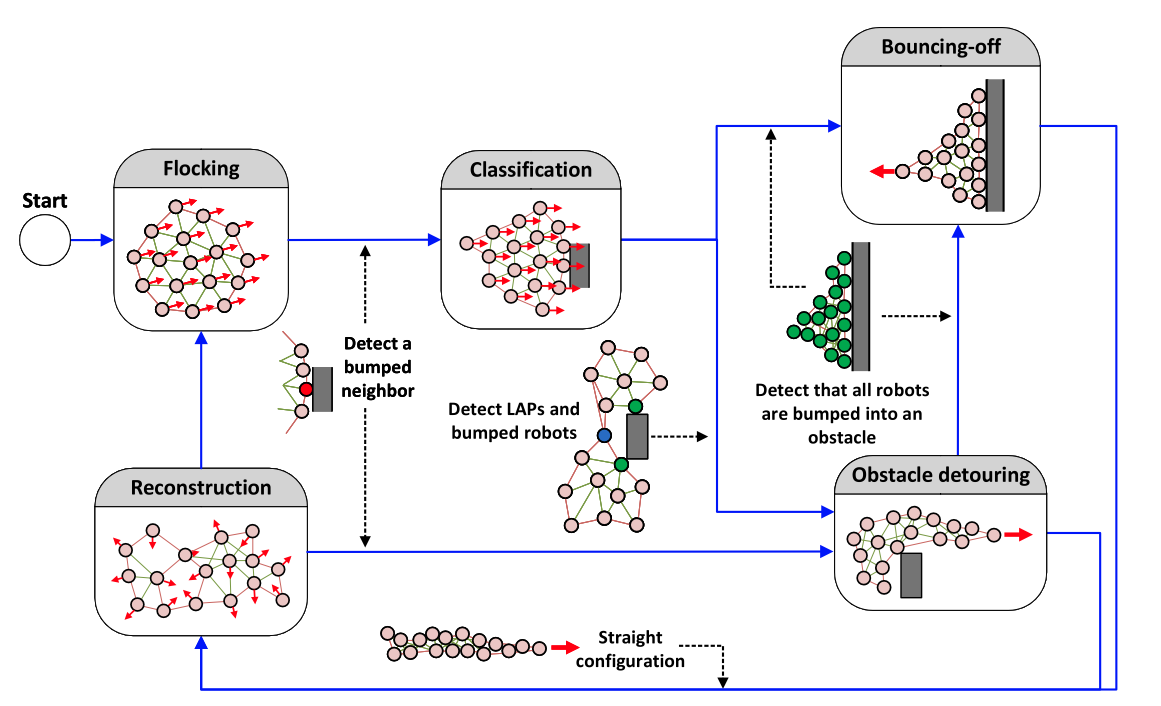
\includegraphics[width=5.5in]{images/Screenshot 2023-02-20 at 1.02.59 PM.png}
    \subsection{Zustand: Classification}

Die Ausgangssituation ist, dass der Schwarm 'flockt', sich also einfach im Raum bewegt und perfekt
ausgerichtet ist.
Wenn ein Roboter nun kollidiert, und kein Nachbar als Hindernis festgestellt werden konnte, geht der
Schwarm in den Classification Zustand über. Der Schwarm tastet nun nach und nach die Größe des Hindernisses
ab, indem geprüft wird, ob noch Roboter existieren, die nicht kollidiert sind. Sind alle Roboter kollidiert
geht der Schwarm über in den Bouncing-off Zustand. Wurde ein Weg ohne weitere Kollisionen gefunden geht
der Schwarm in den Obstacle Detouring Zustand über. Der lokale Gelenkpunkt spielt hier eine Rolle in der
Ermittlung der Größe eines Hindernisses, da ein LGP zwischen zwei kollidierten Nachbarn ein Indikator für
ein 'Map'-Größe ist. Die Kommmunikation im Schwarm ist kostengünstig, da nur zwei Werte übermittelt werden:
isLGP, also ob ein Roboter ein lokaler Gelenkpunkt ist, und ob ein Roboter kollidiert ist.
    \subsection{Zustand: Obstalce Detouring}
    \subsection{Zustand: Bouncing-off}

Wie wir bereits wissen wird sich der Schwarm von einem Hindernis oder einer Wand abstoßen, wenn alle
Roboter kollidiert sind. Das Vorgehen ist relativ simpel und kann der folgenden Abbildung entnommen werden.\\

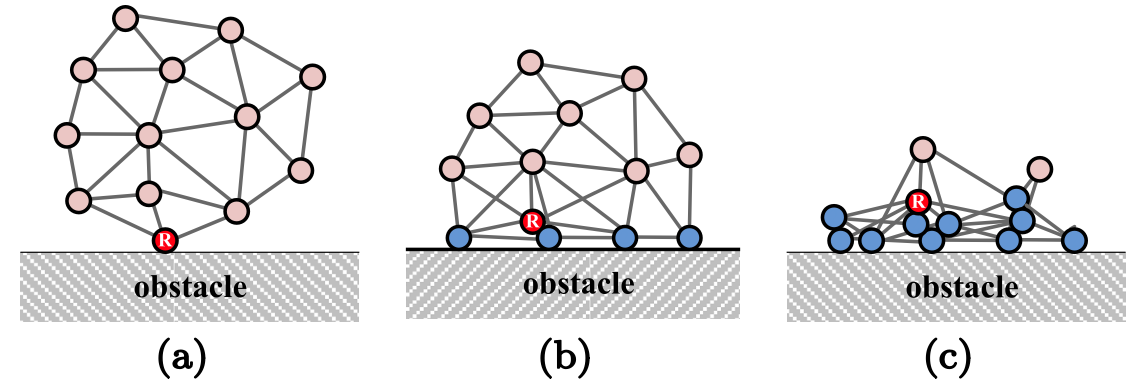
\includegraphics[width=3in]{images/Screenshot 2023-02-20 at 1.32.00 PM.png}
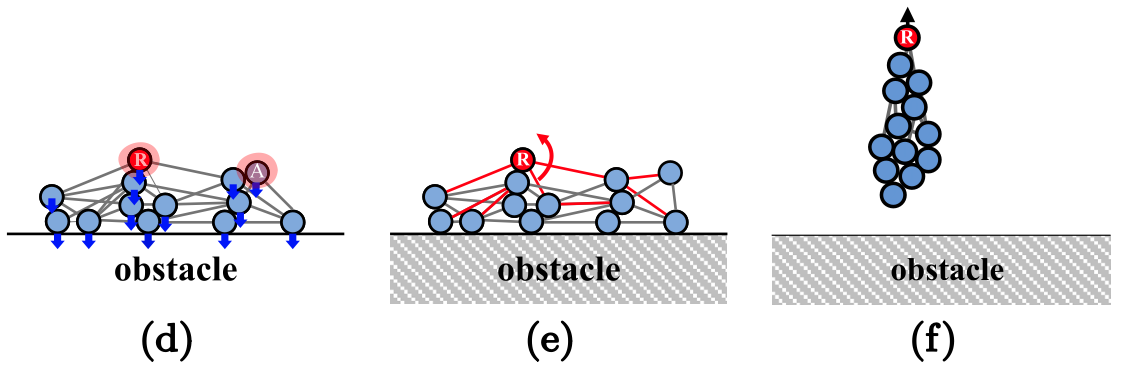
\includegraphics[width=3in]{images/Screenshot 2023-02-20 at 1.32.24 PM.png}

Von Schritt (a) zu Schritt (d) sehen wir, wie alle Roboter kollidieren, der Schwarm befindet sich ab dem
Zeitpunkt zwischen (d) und (e) also im Bouncing-off Zustand. Der Schwarm wählt nun ähnlich wie im Detouring
Zustand den Roboter aus, der am weitesten hinten im Schwarm ist. Das Kriterium, dass dieser Kandidat nicht
kollidiert sein darf, entfällt logischerweise. Dieser neue Lead dreht sich nun vom Hindernis weg und die
anderen Roboter folgen wieder in einer Eltern-Kind-Beziehung. Wurde der maximale Baumwinkel wieder
unterschritten und ist kein Roboter mehr kollidiert, geht der Schwarm auch hier in den Reconstruction Zustand
über.
    \subsection{Zustand: Reconstruction}

    \section{Simulationsergebnisse}

    \section{Schluss}


\end{document}